\documentclass{article}
\usepackage[utf8]{inputenc}

\title{Lab 1: Passwords and Hashing}
\author{Benny Chen | Lars-Erik Laskey}
\date{September 10, 2022}

\usepackage{color}
\usepackage{amsthm}
\usepackage{amssymb} 
\usepackage{amsmath}
\usepackage{listings}
\usepackage{xcolor}
\usepackage{listings}
\usepackage{graphicx}
\usepackage[hidelinks]{hyperref}

\definecolor{codegreen}{rgb}{0,0.6,0}
\definecolor{codegray}{rgb}{0.5,0.5,0.5}
\definecolor{codepurple}{rgb}{0.58,0,0.82}
\definecolor{backcolour}{rgb}{0.95,0.95,0.92}

\lstdefinestyle{mystyle}{
    backgroundcolor=\color{backcolour},   
    commentstyle=\color{codegreen},
    keywordstyle=\color{magenta},
    numberstyle=\tiny\color{codegray},
    stringstyle=\color{codepurple},
    basicstyle=\ttfamily\footnotesize,
    breakatwhitespace=false,         
    breaklines=true,                 
    captionpos=b,                    
    keepspaces=true,                 
    numbers=left,                    
    numbersep=5pt,                  
    showspaces=false,                
    showstringspaces=false,
    showtabs=false,                  
    tabsize=2
}

\lstset{style=mystyle}

\begin{document}

\maketitle

\section{Question 1}
\subsection*{Background:}
As a Connecticut law-enforcement cybersec researcher, you are asked to help find the 
password to the account of Adam Lanza, a dangerous criminal, in the darknet server of Adam’s gang. 
Adam’s username is simply his first name, Adam.Since Adam didn’t study cybersecurity and is known 
for cruelty rather than intelligence, you decide he is likely to use one of these very common passwords.

\subsection*{Task:}
Given a list of most common passwords and a name, Adam, create a script to 
find out what password he used.

\subsubsection*{Break1.py:}
\begin{lstlisting}[language=Python]
    import time
    import os

    if __name__ in '__main__':
    start_time = time.time()
    print("Start time: 0.0")
    common_passwords=[i.strip() for i in open('MostCommonPWs.txt')]

    for i in common_passwords:
        res = os.system('python3 ./Login.pyc'+ ' Adam ' + i + " >/dev/null 2>&1")
        if res == 0:
            print('Adam',i, "--- %s seconds ---" % (time.time() - start_time))
\end{lstlisting}

\subsubsection*{Output:}
\begin{center}
    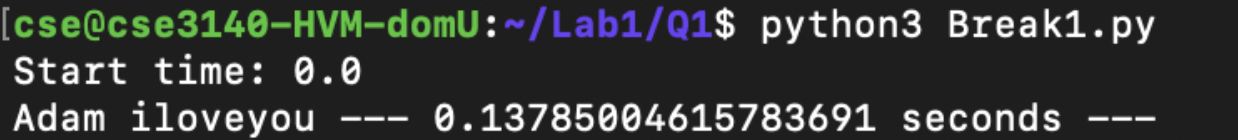
\includegraphics[scale=.55]{images/Q1_Output.png}    
\end{center}


\section{Question 2}

\subsection*{Task:}
Given a list of most common passwords and a list of names, create a script to
find out what passwords they used.

\subsubsection*{Break2.py:}
\begin{lstlisting}[language=Python]
    import time
    import os

    if __name__ in '__main__':
        start_time = time.time()
        common_passwords=[i.strip() for i in open('/home/cse/Lab1/MostCommonPWs.txt')]
        gang_names=[i.strip() for i in open('/home/cse/Lab1/gang.txt')]

        for name in gang_names:
            for i in common_passwords:
                res = os.system('python3 ./Login.pyc'+ ' ' + name + ' ' + i + " >/dev/null 2>&1")
                if res == 0:
                    print(name, i, "--- %s seconds ---" % (time.time() - start_time))
                    break
            if res != 0:
                print(name,' ?')
\end{lstlisting}
\subsubsection*{Output:}
\begin{center}
    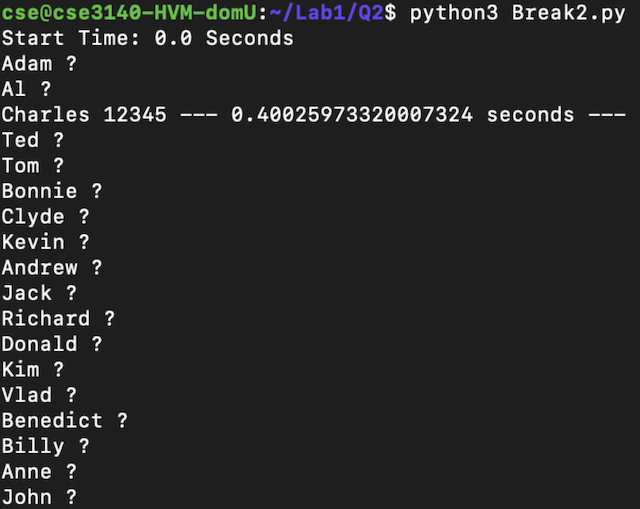
\includegraphics[scale=.8]{images/Q2_Output.png}
\end{center}

\section{Question 3}
\subsection*{Task:}
Given a larger list of most common passwords (of 100k passwords) and a list of names, 
create a script to find out what passwords they used.

\subsection*{Break3.py:}
TODO
\subsection*{Output:}
TODO
\section{Question 4}
\subsection*{Task:}
Given a list of leaked passwords from a site and a list of names, create a script to
find out what passwords they used.

\subsubsection*{Break4.py:}
\begin{lstlisting}[language=Python]
    import time
    import os

    if __name__ in '__main__':
        start_time = time.time()
        leaked_passwords=[(i.strip()) for i in open('/home/cse/Lab1/Q4/PwnedPWfile')]
        gang_names=[i.strip() for i in open('/home/cse/Lab1/gang.txt')]
        leaked_passwords = dict(i.split(',') for i in leaked_passwords)

        for name in gang_names:
            if name in leaked_passwords:
                if os.system('python3 ./Login.pyc ' + name + ' ' + leaked_passwords[name] + " >/dev/null 2>&1") == 0:
                    print(name, leaked_passwords[name], "--- %s seconds ---" % (time.time() - start_time))
\end{lstlisting}

\subsubsection*{Output:}
\begin{center}
    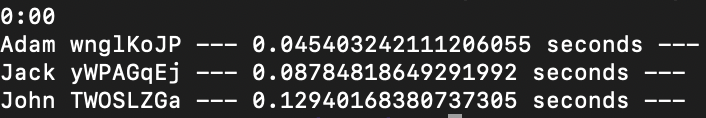
\includegraphics[scale=.5]{images/Q4_Output.png}
\end{center}

\section{Question 5}
\subsection*{Task:}
TODO
\subsubsection*{Break5.py:}
TODO
\subsubsection*{Output:}
TODO
\section{Question 6}
\subsection*{Task:}
TODO
\subsubsection*{Break6.py:}
TODO
\subsubsection*{Output:}
TODO
\section{Question 7}
\subsection*{Task:}
Check if one of your own personal accounts has any exposed passwords using 
\href{https://haveibeenpwned.com/}{haveibeenpwned.com}

\begin{center}
    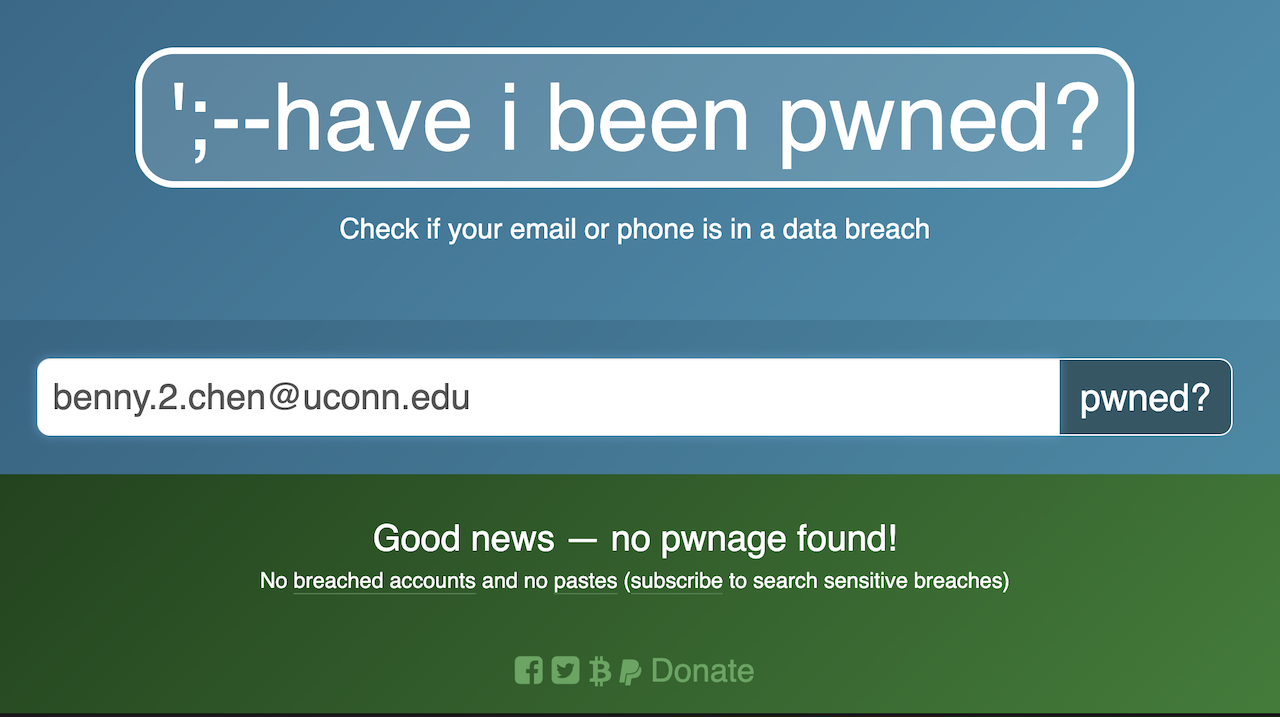
\includegraphics[scale=.5]{images/account_check.png}
    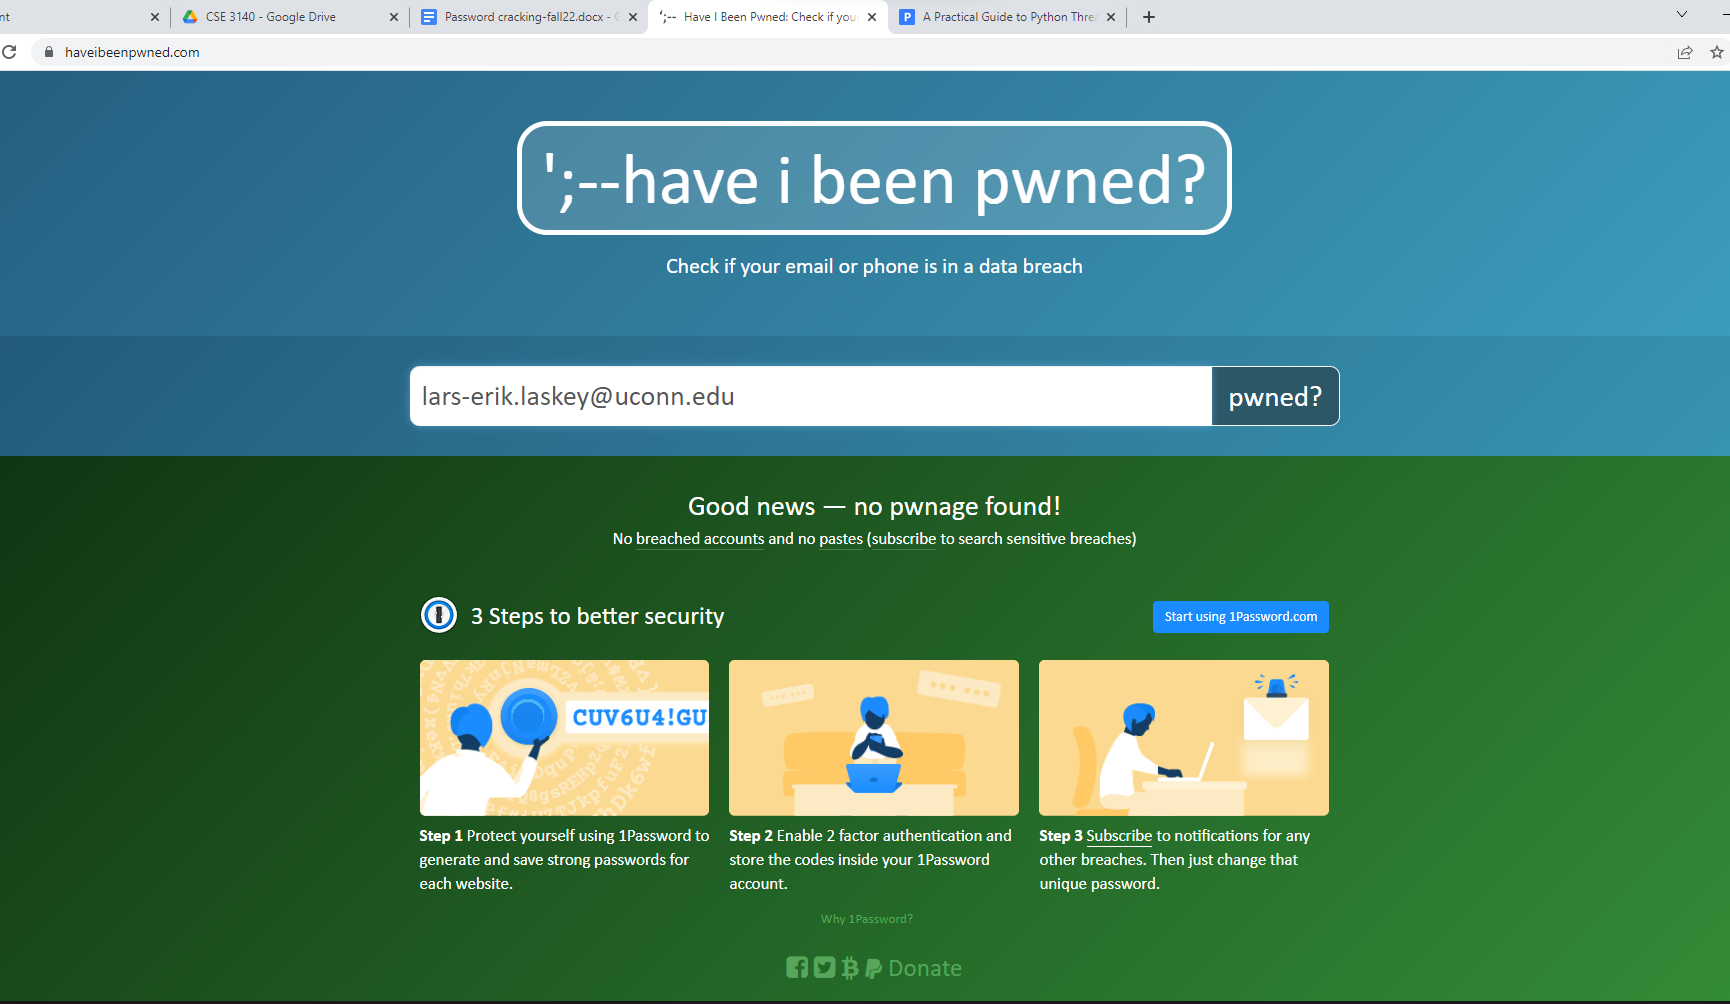
\includegraphics[scale=.245]{images/account_check2.png}
\end{center}

\section{Question 8}
\subsection*{Task:}
Find 2 incidents of web services that have been compromised before.
One by just storing un-hashed passwords in plain text and one hashed but not salted.

\subsubsection*{Incident 1:}
One of the biggest incidents of a service that stored passwords in plain text was actaully
with one of the biggest social media sites, Facebook. In early 2019, a routine secuity review
found that Facebook had stored passwords in plain unhashed text for years. This was a huge
security breach as it meant that anyone with access to the database could easily access the
passwords of millions of users. According to Facebook, they could not find any evidence that
anyone had accessed the passwords for malicious use, but it was still a huge security breach. The passwords were
stored in plain text because Facebook had a legacy system that was not updated to store passwords
in a more secure way. This incident was a huge security breach and Facebook was fined 5 billion
for it.

\begin{center}
    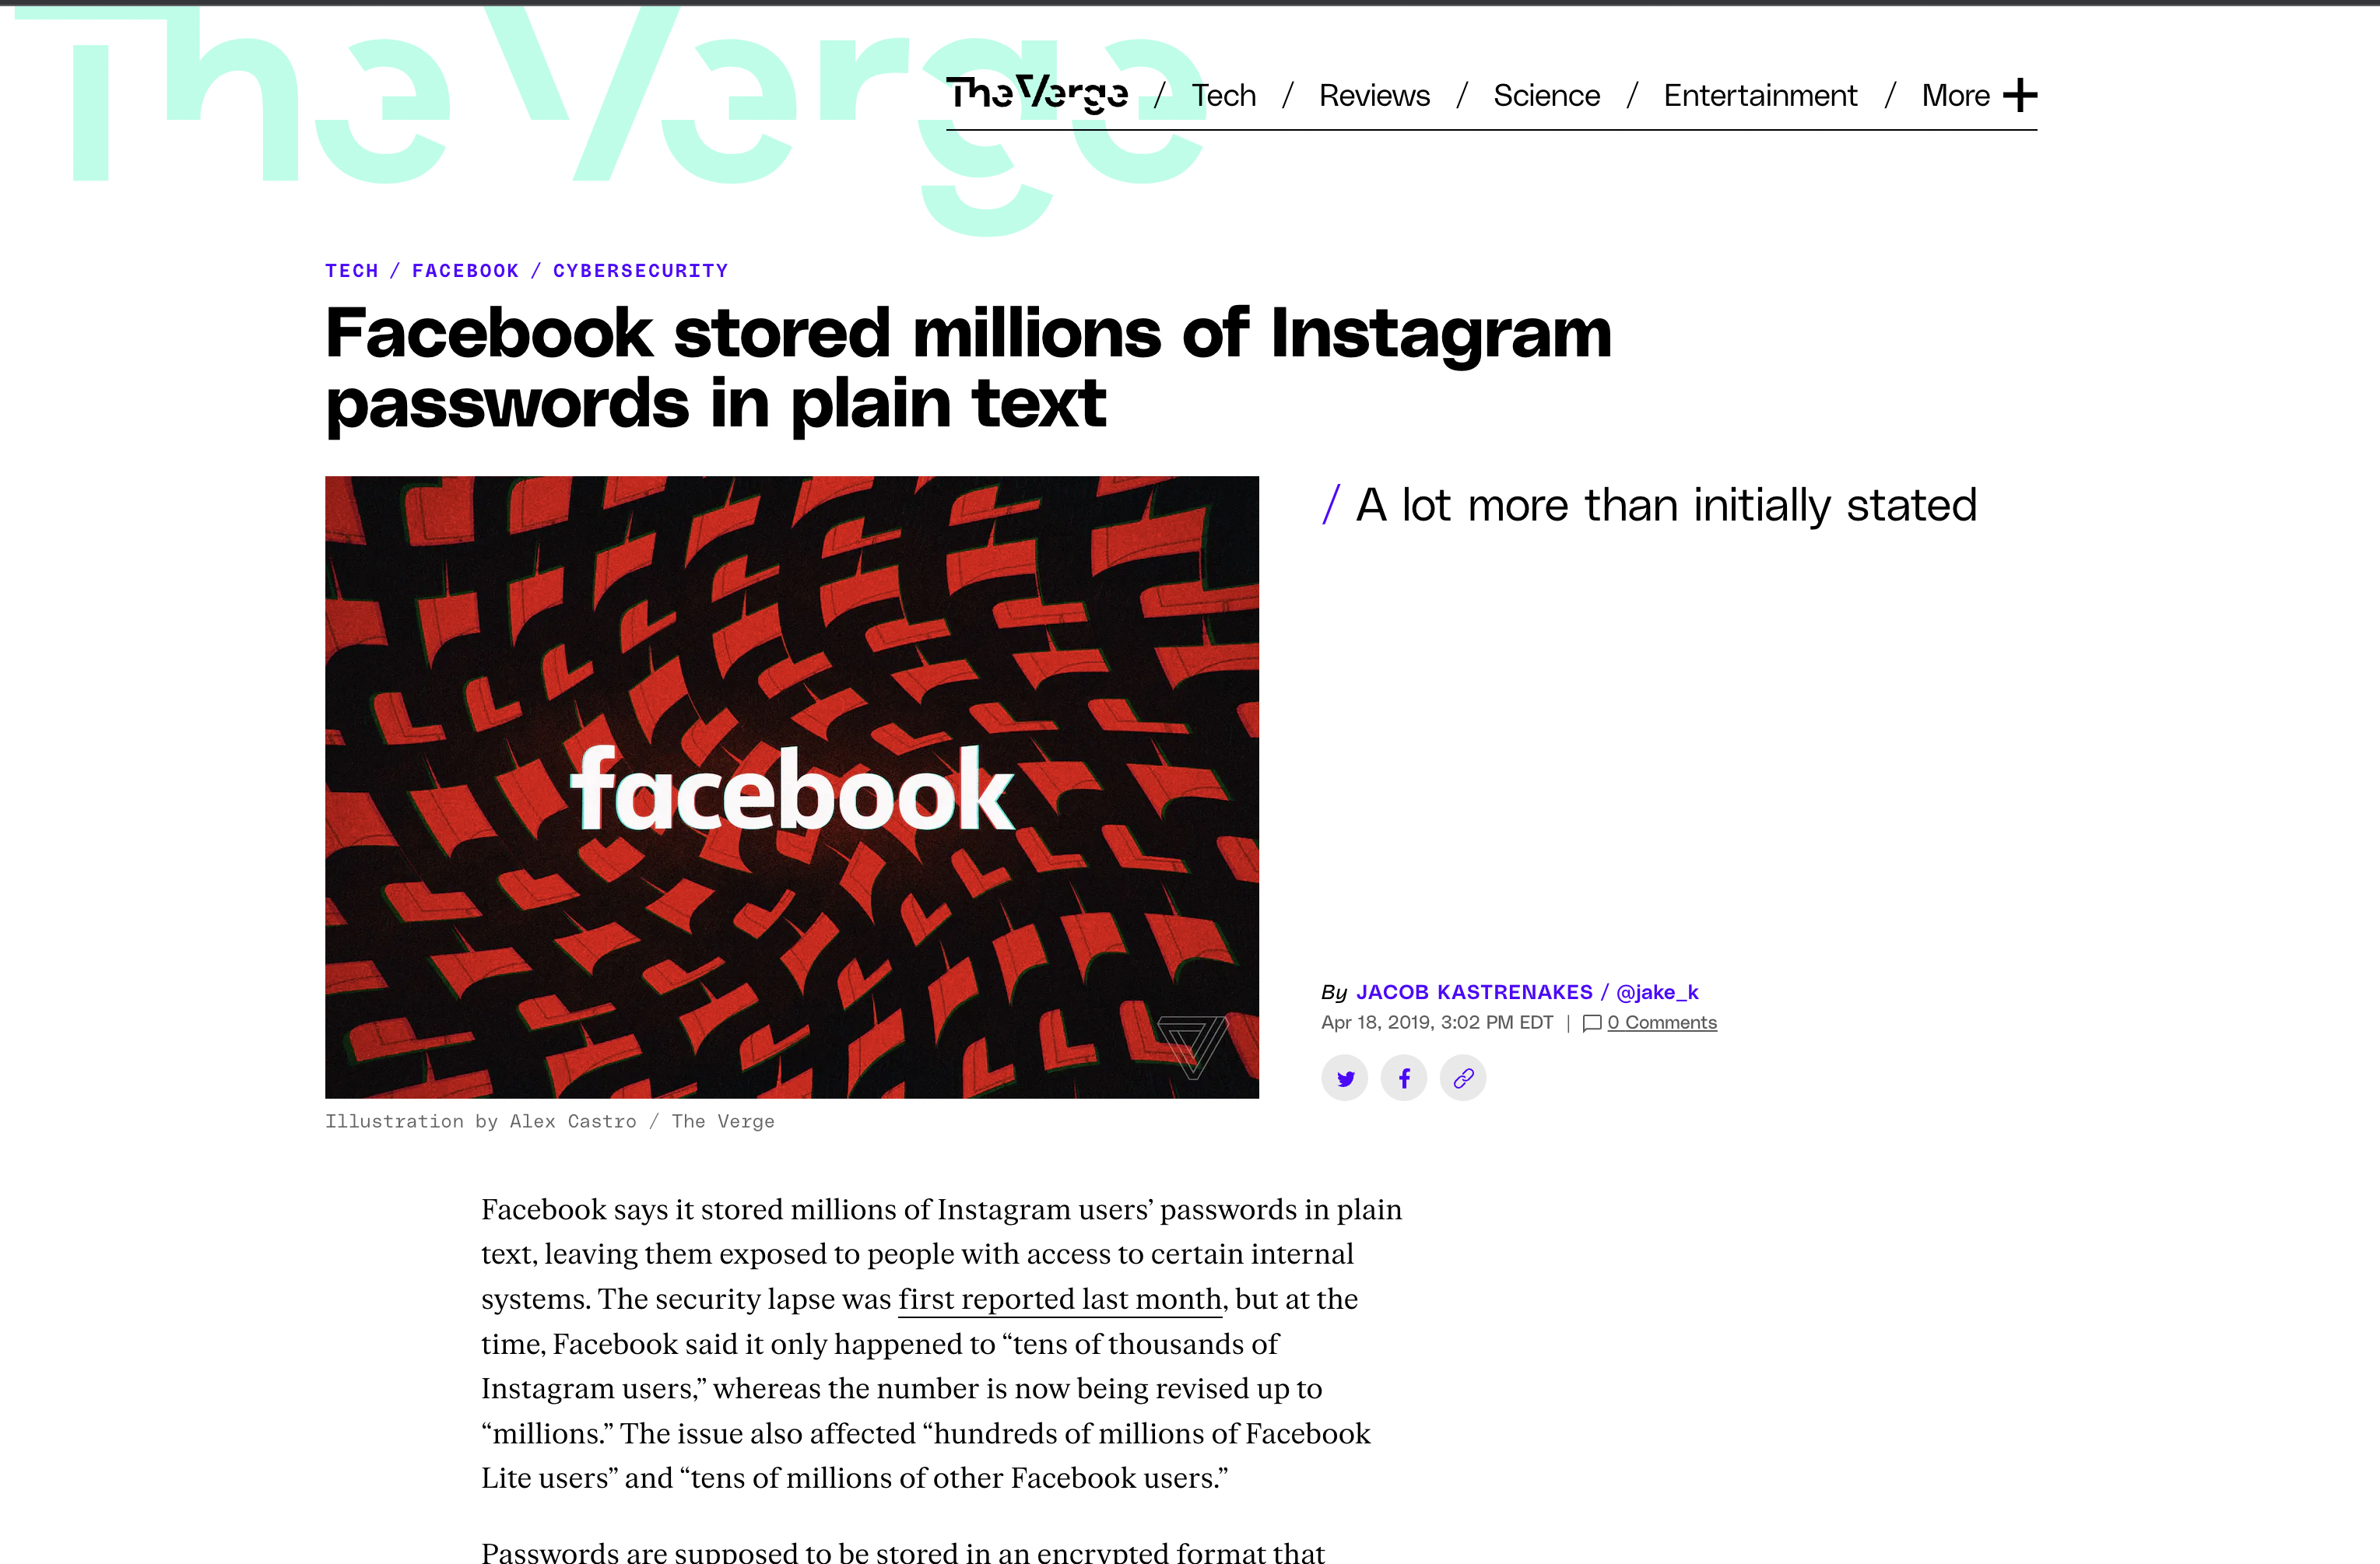
\includegraphics[scale=.22]{images/verge_source.png}
    link: https://www.theverge.com/2019/4/18/18485599/facebook-instagram-passwords-plain-text-millions-users
\end{center}

\subsubsection*{Incident 2:}
Another incident was with the popular job search and career development site, LinkedIn. 
In 2012, LinkedIn was hacked and 6.5 million passwords were stolen. The passwords were stored
and hashed using the SHA-1 algorithm, but were not salted. This means that the passwords were
hashed using a one-way function, but the same password would always hash to the same value.
This made it easy for attackers to crack the passwords. 

\section{Question 9}
\subsection*{Task:} Give an example of a website that does not support or offer 2FA.

\subsection*{Example:}
Even though 2FA is not a perfect solution, it is still a good way to protect your account. 
There are many websites that now support 2FA and are moving towards it, making it a standard.
However, there are still many websites that do not support 2FA. A couple fields that are still
not using 2FA are the utilities and entertainment fields. One example of a website that does
not support 2FA is the popular video streaming service, Netflix. Netflix does not support 2FA
and does not offer it as an option. This is a huge security risk as there is only one layer of
protection for your account and if your password is compromised, your account is compromised.
A example in the utilities field is Connecticut's Electric and Gas company, Eversource. Eversource
does not offer 2FA which should be crucial for a company that handles sensitive information
such as credit card numbers and social security numbers. 
\end{document}